\documentclass[a4paper,5pt]{amsbook}
%%%%%%%%%%%%%%%%%%%%%%%%%%%%%%%%%%%%%%%%%%%%%%%%%%%%%%%%%%%%%%%%%%%%%

\usepackage{booktabs}
\usepackage{graphicx}
\usepackage{multicol}
\usepackage{textcomp}
\usepackage{systeme}
\usepackage{amssymb}
\usepackage{amsmath}
\usepackage{subcaption}
\usepackage[inline]{enumitem}
\usepackage[portuguese]{babel}

%%%%%%%%%%%%%%%%%%%%%%%%%%%%%%%%%%%%%%%%%%%%%%%%%%%%%%%%%%%%%%

\newcommand{\sen}{\,\mbox{sen}\,}
\newcommand{\tg}{\,\mbox{tg}\,}
\newcommand{\cosec}{\,\mbox{cosec}\,}
\newcommand{\cotg}{\,\mbox{cotg}\,}
\newcommand{\tr}{\,\mbox{tr}\,}
\newcommand{\ds}{\displaystyle}

%%%%%%%%%%%%%%%%%%%%%%%%%%%%%%%%%%%%%%%%%%%%%%%%%%%%%%%%%%%%%%%%%%%%%%%%

\setlength{\textwidth}{16cm} %\setlength{\topmargin}{-1.3cm}
\setlength{\textheight}{26cm}
\setlength{\leftmargin}{1.2cm} \setlength{\rightmargin}{1.2cm}
\setlength{\oddsidemargin}{0cm}\setlength{\evensidemargin}{0cm}
\setlength{\topmargin}{-1cm}

%%%%%%%%%%%%%%%%%%%%%%%%%%%%%%%%%%%%%%%%%%%%%%%%%%%%%%%%%%%%%%%%%%%%%%%%

% \renewcommand{\baselinestretch}{1.6}
% \renewcommand{\thefootnote}{\fnsymbol{footnote}}
% \renewcommand{\theequation}{\thesection.\arabic{equation}}
% \setlength{\voffset}{-50pt}
% \numberwithin{equation}{chapter}

%%%%%%%%%%%%%%%%%%%%%%%%%%%%%%%%%%%%%%%%%%%%%%%%%%%%%%%%%%%%%%%%%%%%%%%

\begin{document}
\thispagestyle{empty}
\pagestyle{empty}
\begin{minipage}[h]{0.14\textwidth}
	
\includegraphics[scale=0.24]{../../ufgd.png}
\end{minipage}
\begin{minipage}[h]{\textwidth}
\begin{tabular}{c}
{{\bf UNIVERSIDADE FEDERAL DA GRANDE DOURADOS}}\\
{{\bf Geometria --- Lista 5}}\\
{{\bf Prof.\ Adriano Barbosa}}\\
\end{tabular}
\vspace{-0.45cm}
%
\end{minipage}

%------------------------

\vspace{1cm}
%%%%%%%%%%%%%%%%%%%%%%%%%%%%%%%%   formulario  inicio  %%%%%%%%%%%%%%%%%%%%%%%%%%%%%%%%
\begin{enumerate}
    \item No paralelep\'{\i}pedo reto ret\^angulo da figura, calcule a dist\^ancia do
        v\'ertice $C$ ao segmento $AM$, sendo $M$ o ponto m\'edio de $CE$.
        \begin{figure}[!h]
            \centering
            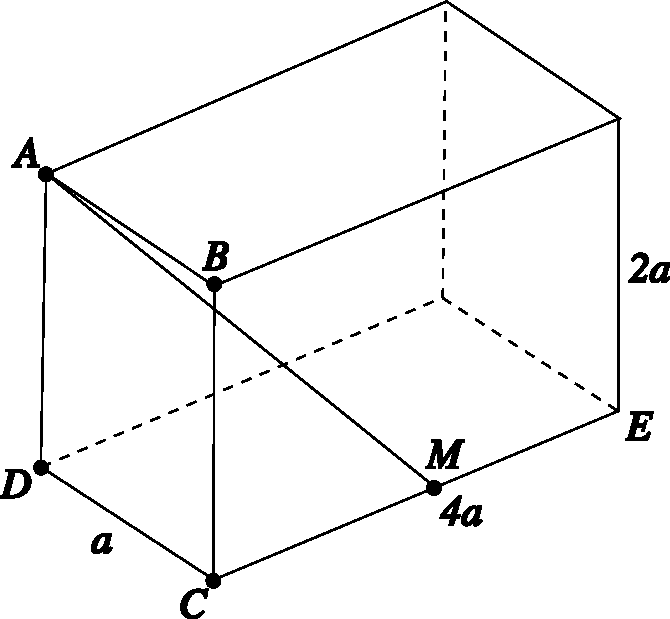
\includegraphics[width=0.3\textwidth]{fig05-1.pdf}
        \end{figure}

    \item Considere o tri\^angulo is\'osceles $ABC$, representado pela figura
        abaixo, cujos lados congruentes $AB$ e $AC$ medem 5. Assuma que o
        terceiro lado e o \^angulo oposto a este lado sejam vari\'aveis, medindo
        $\overline{BC}=x$ e $\hat{A}=\theta$, respectivamente.
        \begin{enumerate}
            \vspace{0.3cm}
            \item Encontre a fun\c{c}\~ao que expressa a \'area do tri\^angulo $ABC$ em
                fun\c{c}\~ao do \^angulo $\theta$, indicando o dom\'{\i}nio e a express\~ao
                da fun\c{c}\~ao.
            \vspace{0.3cm}
            \item Calcule a \'area m\'axima do tri\^angulo. Quais as medidas de $x$ e
                $\theta$ neste caso?
        \end{enumerate}
        \begin{figure}[!h]
            \centering
            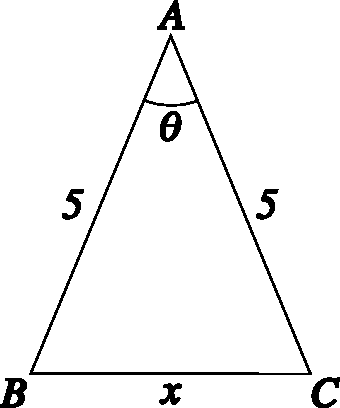
\includegraphics[width=0.17\textwidth]{fig05-2.pdf}
        \end{figure}

    \item Dados uma esfera $\Gamma$ de centro $O$ e raio $r$, e um ponto $P$,
        com $\overline{OP} = d>r$.
        \begin{enumerate}
            \vspace{0.3cm}
            \item Para $T\in\Gamma$, mostre que a reta
                $\overleftrightarrow{PT}$ \'e tangente a $\Gamma$ se, e somente
                se, $\overline{PT} = \sqrt{d^2-r^2}$.
            \vspace{0.3cm}
            \item Mostre que o lugar geom\'etrico dos pontos $T\in\Gamma$ tais
                que $\overleftrightarrow{PT}$ \'e tangente a $\Gamma$ est\'a
                contido em um c\'{\i}rculo, determinando seu centro, raio e o plano
                em que est\'a contido.
        \end{enumerate}
        \begin{figure}[!h]
            \centering
            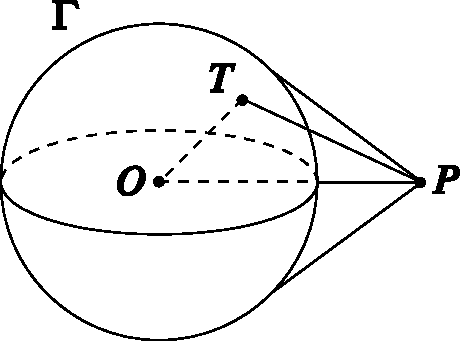
\includegraphics[width=0.3\textwidth]{fig05-3.pdf}
        \end{figure}

    \newpage
    \item Considere o quadril\'atero convexo abaixo, representado com suas
        diagonais. As letras correspondem \`as medidas dos segmentos e $0^\circ <
        \theta \le 90^\circ$ representa um dos \^angulos entre as diagonais.
        \begin{enumerate}
            \vspace{0.3cm}
            \item Se $\theta = 90^\circ$, prove que $a^2+c^2 = b^2+d^2$.
            \vspace{0.3cm}
            \item Se $a^2+c^2 = b^2+d^2$, prove que $(xw+yz)\cos\theta =
                -(xy+zw)\cos\theta$.
            \vspace{0.3cm}
            \item Se $a^2+c^2 = b^2+d^2$, prove que $\theta = 90^\circ$.
        \end{enumerate}
        \begin{figure}[!h]
            \centering
            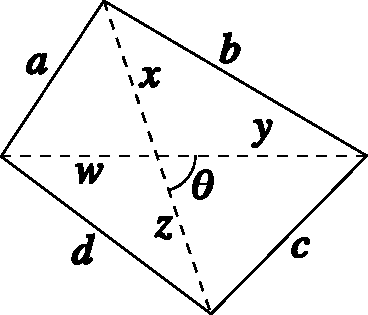
\includegraphics[width=0.3\textwidth]{fig05-4.pdf}
        \end{figure}

    \item Nos dois casos abaixo, demonstre a conhecida rela\c{c}\~ao m\'etrica
        $\overline{PA} \cdot \overline{PB} = \overline{PC} \cdot
        \overline{PD}$, tamb\'em chamada de ``pot\^encia de ponto no c\'{\i}rculo'':
        \begin{enumerate}
            \vspace{0.3cm}
            \item $P$ exterior ao c\'{\i}rculo (figura da esquerda).
            \vspace{0.3cm}
            \item $P$ interior ao c\'{\i}rculo (figura da direita).
        \end{enumerate}
        \begin{figure}[!h]
            \centering
            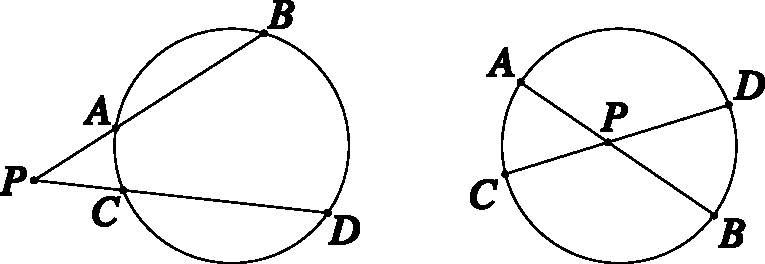
\includegraphics[width=0.5\textwidth]{fig05-5.pdf}
        \end{figure}
\end{enumerate}

\end{document}
